\documentclass[twoside]{book}

% Packages required by doxygen
\usepackage{fixltx2e}
\usepackage{calc}
\usepackage{doxygen}
\usepackage[export]{adjustbox} % also loads graphicx
\usepackage{graphicx}
\usepackage[utf8]{inputenc}
\usepackage{makeidx}
\usepackage{multicol}
\usepackage{multirow}
\PassOptionsToPackage{warn}{textcomp}
\usepackage{textcomp}
\usepackage[nointegrals]{wasysym}
\usepackage[table]{xcolor}

% Font selection
\usepackage[T1]{fontenc}
\usepackage[scaled=.90]{helvet}
\usepackage{courier}
\usepackage{amssymb}
\usepackage{sectsty}
\renewcommand{\familydefault}{\sfdefault}
\allsectionsfont{%
  \fontseries{bc}\selectfont%
  \color{darkgray}%
}
\renewcommand{\DoxyLabelFont}{%
  \fontseries{bc}\selectfont%
  \color{darkgray}%
}
\newcommand{\+}{\discretionary{\mbox{\scriptsize$\hookleftarrow$}}{}{}}

% Page & text layout
\usepackage{geometry}
\geometry{%
  a4paper,%
  top=2.5cm,%
  bottom=2.5cm,%
  left=2.5cm,%
  right=2.5cm%
}
\tolerance=750
\hfuzz=15pt
\hbadness=750
\setlength{\emergencystretch}{15pt}
\setlength{\parindent}{0cm}
\setlength{\parskip}{3ex plus 2ex minus 2ex}
\makeatletter
\renewcommand{\paragraph}{%
  \@startsection{paragraph}{4}{0ex}{-1.0ex}{1.0ex}{%
    \normalfont\normalsize\bfseries\SS@parafont%
  }%
}
\renewcommand{\subparagraph}{%
  \@startsection{subparagraph}{5}{0ex}{-1.0ex}{1.0ex}{%
    \normalfont\normalsize\bfseries\SS@subparafont%
  }%
}
\makeatother

% Headers & footers
\usepackage{fancyhdr}
\pagestyle{fancyplain}
\fancyhead[LE]{\fancyplain{}{\bfseries\thepage}}
\fancyhead[CE]{\fancyplain{}{}}
\fancyhead[RE]{\fancyplain{}{\bfseries\leftmark}}
\fancyhead[LO]{\fancyplain{}{\bfseries\rightmark}}
\fancyhead[CO]{\fancyplain{}{}}
\fancyhead[RO]{\fancyplain{}{\bfseries\thepage}}
\fancyfoot[LE]{\fancyplain{}{}}
\fancyfoot[CE]{\fancyplain{}{}}
\fancyfoot[RE]{\fancyplain{}{\bfseries\scriptsize Generated by Doxygen }}
\fancyfoot[LO]{\fancyplain{}{\bfseries\scriptsize Generated by Doxygen }}
\fancyfoot[CO]{\fancyplain{}{}}
\fancyfoot[RO]{\fancyplain{}{}}
\renewcommand{\footrulewidth}{0.4pt}
\renewcommand{\chaptermark}[1]{%
  \markboth{#1}{}%
}
\renewcommand{\sectionmark}[1]{%
  \markright{\thesection\ #1}%
}

% Indices & bibliography
\usepackage{natbib}
\usepackage[titles]{tocloft}
\setcounter{tocdepth}{3}
\setcounter{secnumdepth}{5}
\makeindex

% Hyperlinks (required, but should be loaded last)
\usepackage{ifpdf}
\ifpdf
  \usepackage[pdftex,pagebackref=true]{hyperref}
\else
  \usepackage[ps2pdf,pagebackref=true]{hyperref}
\fi
\hypersetup{%
  colorlinks=true,%
  linkcolor=blue,%
  citecolor=blue,%
  unicode%
}

% Custom commands
\newcommand{\clearemptydoublepage}{%
  \newpage{\pagestyle{empty}\cleardoublepage}%
}

\usepackage{caption}
\captionsetup{labelsep=space,justification=centering,font={bf},singlelinecheck=off,skip=4pt,position=top}

%===== C O N T E N T S =====

\begin{document}

% Titlepage & ToC
\hypersetup{pageanchor=false,
             bookmarksnumbered=true,
             pdfencoding=unicode
            }
\pagenumbering{alph}
\begin{titlepage}
\vspace*{7cm}
\begin{center}%
{\Large My Project }\\
\vspace*{1cm}
{\large Generated by Doxygen 1.8.12}\\
\end{center}
\end{titlepage}
\clearemptydoublepage
\pagenumbering{roman}
\tableofcontents
\clearemptydoublepage
\pagenumbering{arabic}
\hypersetup{pageanchor=true}

%--- Begin generated contents ---
\chapter{Hierarchical Index}
\section{Class Hierarchy}
This inheritance list is sorted roughly, but not completely, alphabetically\+:\begin{DoxyCompactList}
\item \contentsline{section}{Card}{\pageref{class_card}}{}
\begin{DoxyCompactList}
\item \contentsline{section}{Inherete}{\pageref{class_inherete}}{}
\end{DoxyCompactList}
\item \contentsline{section}{dealer}{\pageref{structdealer}}{}
\item \contentsline{section}{player}{\pageref{structplayer}}{}
\end{DoxyCompactList}

\chapter{Class Index}
\section{Class List}
Here are the classes, structs, unions and interfaces with brief descriptions\+:\begin{DoxyCompactList}
\item\contentsline{section}{\hyperlink{structdealer}{dealer} }{\pageref{structdealer}}{}
\item\contentsline{section}{\hyperlink{structplayer}{player} }{\pageref{structplayer}}{}
\end{DoxyCompactList}

\chapter{File Index}
\section{File List}
Here is a list of all files with brief descriptions\+:\begin{DoxyCompactList}
\item\contentsline{section}{C\+:/\+Users/\+Jose/\+Desktop/\+C\+S\+C17\+A/\+Proj/blk\+Jk2/\hyperlink{_8dep_8inc}{.\+dep.\+inc} }{\pageref{_8dep_8inc}}{}
\item\contentsline{section}{C\+:/\+Users/\+Jose/\+Desktop/\+C\+S\+C17\+A/\+Proj/blk\+Jk2/\hyperlink{main_8cpp}{main.\+cpp} }{\pageref{main_8cpp}}{}
\item\contentsline{section}{C\+:/\+Users/\+Jose/\+Desktop/\+C\+S\+C17\+A/\+Proj/blk\+Jk2/\hyperlink{playinfo_8h}{playinfo.\+h} }{\pageref{playinfo_8h}}{}
\end{DoxyCompactList}

\chapter{Class Documentation}
\hypertarget{class_card}{}\section{Card Class Reference}
\label{class_card}\index{Card@{Card}}


{\ttfamily \#include $<$Card.\+h$>$}

Inheritance diagram for Card\+:\begin{figure}[H]
\begin{center}
\leavevmode
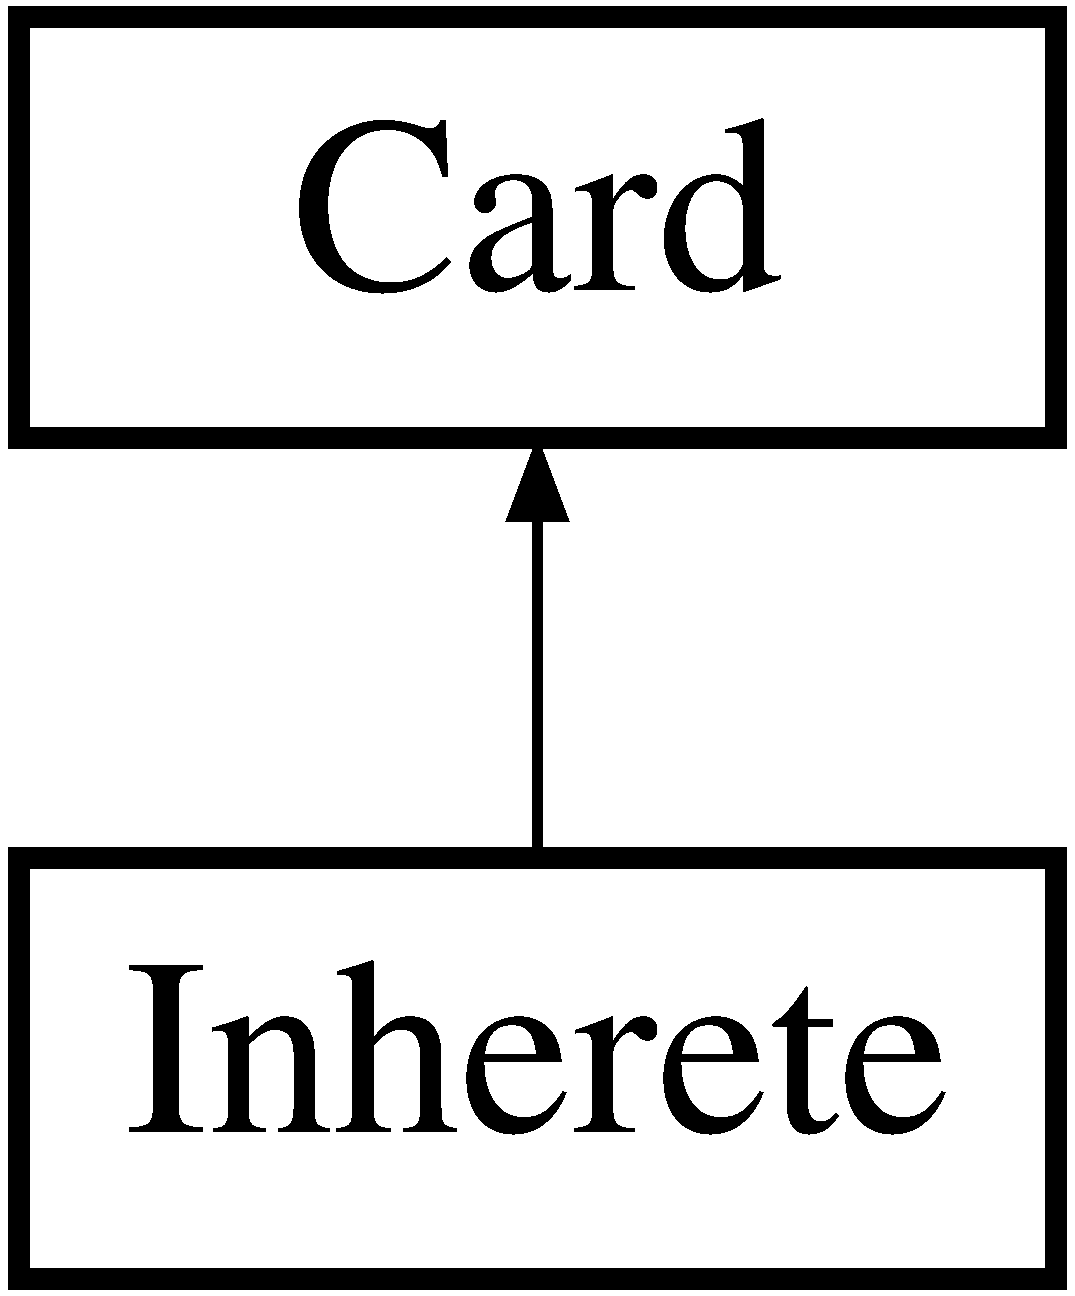
\includegraphics[height=2.000000cm]{class_card}
\end{center}
\end{figure}
\subsection*{Public Member Functions}
\begin{DoxyCompactItemize}
\item 
\hyperlink{class_card_a783f5854cbe8c183ee3d4414c01472c0}{Card} ()
\item 
int \hyperlink{class_card_ab8abc1fb7afe26a4f5be4ae5ce08e936}{value} ()
\item 
char \hyperlink{class_card_a7bbc5f0f0b73077d6f9764f66c6d765a}{suit} ()
\end{DoxyCompactItemize}


\subsection{Constructor \& Destructor Documentation}
\hypertarget{class_card_a783f5854cbe8c183ee3d4414c01472c0}{}\label{class_card_a783f5854cbe8c183ee3d4414c01472c0} 
\index{Card@{Card}!Card@{Card}}
\index{Card@{Card}!Card@{Card}}
\subsubsection{\texorpdfstring{Card()}{Card()}}
{\footnotesize\ttfamily Card\+::\+Card (\begin{DoxyParamCaption}{ }\end{DoxyParamCaption})}



\subsection{Member Function Documentation}
\hypertarget{class_card_a7bbc5f0f0b73077d6f9764f66c6d765a}{}\label{class_card_a7bbc5f0f0b73077d6f9764f66c6d765a} 
\index{Card@{Card}!suit@{suit}}
\index{suit@{suit}!Card@{Card}}
\subsubsection{\texorpdfstring{suit()}{suit()}}
{\footnotesize\ttfamily char Card\+::suit (\begin{DoxyParamCaption}{ }\end{DoxyParamCaption})}

\hypertarget{class_card_ab8abc1fb7afe26a4f5be4ae5ce08e936}{}\label{class_card_ab8abc1fb7afe26a4f5be4ae5ce08e936} 
\index{Card@{Card}!value@{value}}
\index{value@{value}!Card@{Card}}
\subsubsection{\texorpdfstring{value()}{value()}}
{\footnotesize\ttfamily Card\+::value (\begin{DoxyParamCaption}{ }\end{DoxyParamCaption})}



The documentation for this class was generated from the following files\+:\begin{DoxyCompactItemize}
\item 
\hyperlink{_card_8h}{Card.\+h}\item 
\hyperlink{_card_8cpp}{Card.\+cpp}\end{DoxyCompactItemize}

\hypertarget{structdealer}{}\section{dealer Struct Reference}
\label{structdealer}\index{dealer@{dealer}}


{\ttfamily \#include $<$playinfo.\+h$>$}

\subsection*{Public Attributes}
\begin{DoxyCompactItemize}
\item 
unsigned int \hyperlink{structdealer_a219ecd2fac1ba66a587925272daebb44}{value} = 0
\item 
string \hyperlink{structdealer_aad8ef1a02957ef6f542c1cea1f41fc2f}{suit}
\end{DoxyCompactItemize}


\subsection{Member Data Documentation}
\hypertarget{structdealer_aad8ef1a02957ef6f542c1cea1f41fc2f}{}\label{structdealer_aad8ef1a02957ef6f542c1cea1f41fc2f} 
\index{dealer@{dealer}!suit@{suit}}
\index{suit@{suit}!dealer@{dealer}}
\subsubsection{\texorpdfstring{suit}{suit}}
{\footnotesize\ttfamily string dealer\+::suit}

\hypertarget{structdealer_a219ecd2fac1ba66a587925272daebb44}{}\label{structdealer_a219ecd2fac1ba66a587925272daebb44} 
\index{dealer@{dealer}!value@{value}}
\index{value@{value}!dealer@{dealer}}
\subsubsection{\texorpdfstring{value}{value}}
{\footnotesize\ttfamily unsigned int dealer\+::value = 0}



The documentation for this struct was generated from the following file\+:\begin{DoxyCompactItemize}
\item 
C\+:/\+Users/\+Jose/\+Desktop/\+C\+S\+C17\+A/\+Proj/blk\+Jk2/\hyperlink{playinfo_8h}{playinfo.\+h}\end{DoxyCompactItemize}

\hypertarget{class_inherete}{}\section{Inherete Class Reference}
\label{class_inherete}\index{Inherete@{Inherete}}


{\ttfamily \#include $<$Inherete.\+h$>$}

Inheritance diagram for Inherete\+:\begin{figure}[H]
\begin{center}
\leavevmode
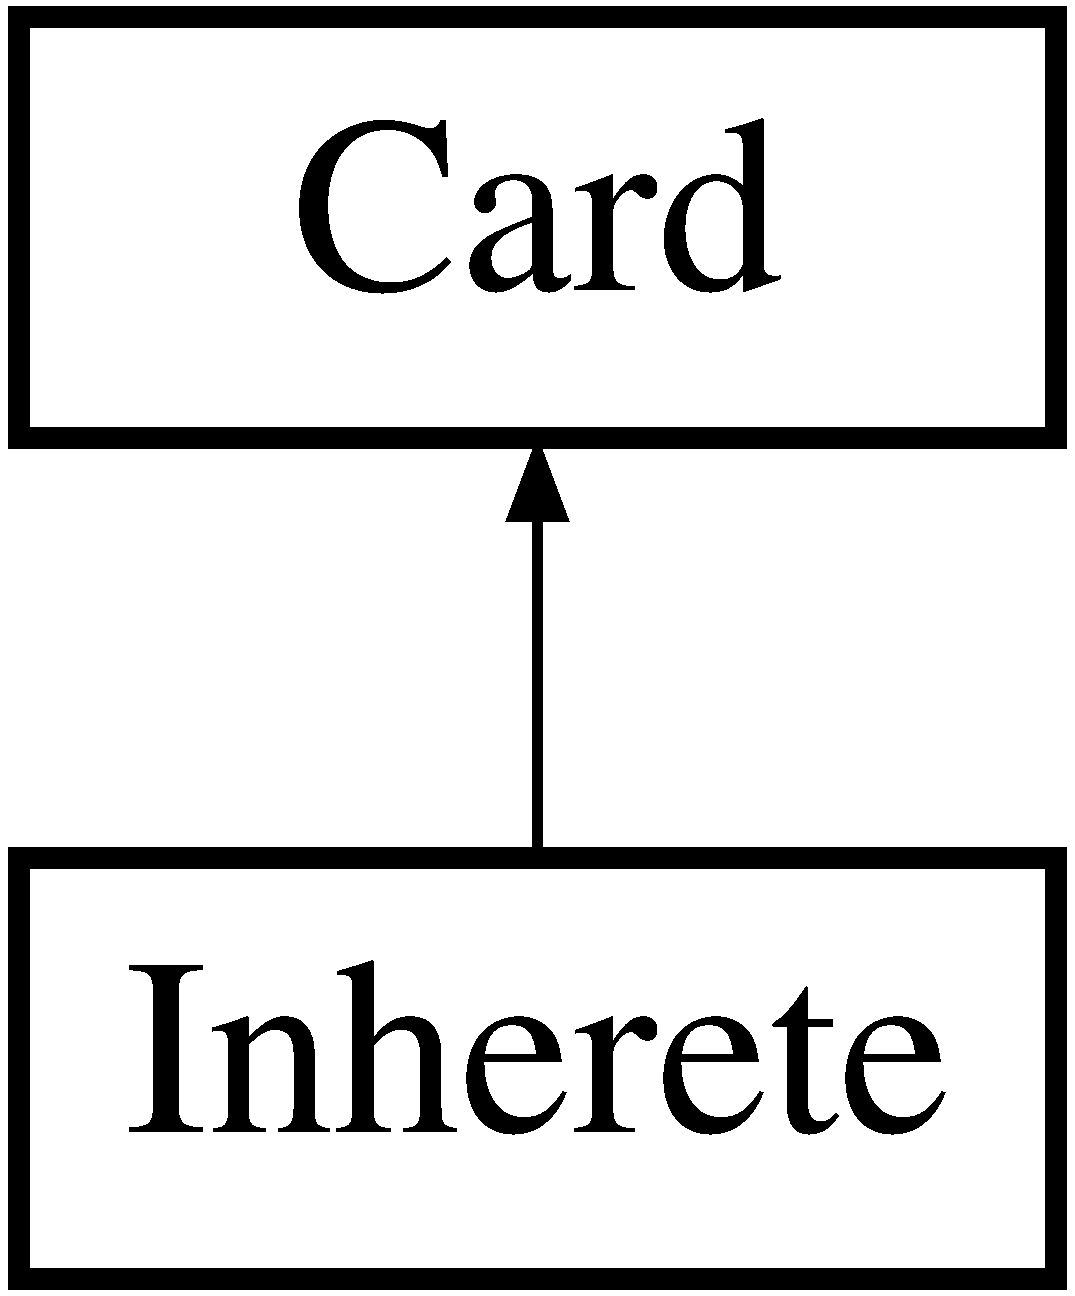
\includegraphics[height=2.000000cm]{class_inherete}
\end{center}
\end{figure}
\subsection*{Public Member Functions}
\begin{DoxyCompactItemize}
\item 
\hyperlink{class_inherete_ad6ec31af18bd655c024e6572dba5dc1b}{Inherete} ()
\item 
void \hyperlink{class_inherete_a0952f09588eed23f2c9ff449d6cb1166}{set\+Test1} (int)
\item 
int \hyperlink{class_inherete_ab68de696572168fd0e000769925c578f}{get\+Test1} ()
\item 
void \hyperlink{class_inherete_ad1f7eeac2bc911bd5746a28648c6a98d}{set\+Test2} (int)
\item 
int \hyperlink{class_inherete_a351b5ccefdd1f0dbe1bfcac0a7f98270}{get\+Test2} ()
\end{DoxyCompactItemize}
\subsection*{Protected Attributes}
\begin{DoxyCompactItemize}
\item 
int \hyperlink{class_inherete_a3c7cd588b0f27f922ab4d8ba62150f80}{test1}
\item 
int \hyperlink{class_inherete_aab5737b7592b7be0f19d1268d86df269}{test2}
\end{DoxyCompactItemize}


\subsection{Constructor \& Destructor Documentation}
\hypertarget{class_inherete_ad6ec31af18bd655c024e6572dba5dc1b}{}\label{class_inherete_ad6ec31af18bd655c024e6572dba5dc1b} 
\index{Inherete@{Inherete}!Inherete@{Inherete}}
\index{Inherete@{Inherete}!Inherete@{Inherete}}
\subsubsection{\texorpdfstring{Inherete()}{Inherete()}}
{\footnotesize\ttfamily Inherete\+::\+Inherete (\begin{DoxyParamCaption}{ }\end{DoxyParamCaption})}



\subsection{Member Function Documentation}
\hypertarget{class_inherete_ab68de696572168fd0e000769925c578f}{}\label{class_inherete_ab68de696572168fd0e000769925c578f} 
\index{Inherete@{Inherete}!get\+Test1@{get\+Test1}}
\index{get\+Test1@{get\+Test1}!Inherete@{Inherete}}
\subsubsection{\texorpdfstring{get\+Test1()}{getTest1()}}
{\footnotesize\ttfamily int Inherete\+::get\+Test1 (\begin{DoxyParamCaption}{ }\end{DoxyParamCaption})}

\hypertarget{class_inherete_a351b5ccefdd1f0dbe1bfcac0a7f98270}{}\label{class_inherete_a351b5ccefdd1f0dbe1bfcac0a7f98270} 
\index{Inherete@{Inherete}!get\+Test2@{get\+Test2}}
\index{get\+Test2@{get\+Test2}!Inherete@{Inherete}}
\subsubsection{\texorpdfstring{get\+Test2()}{getTest2()}}
{\footnotesize\ttfamily int Inherete\+::get\+Test2 (\begin{DoxyParamCaption}{ }\end{DoxyParamCaption})}

\hypertarget{class_inherete_a0952f09588eed23f2c9ff449d6cb1166}{}\label{class_inherete_a0952f09588eed23f2c9ff449d6cb1166} 
\index{Inherete@{Inherete}!set\+Test1@{set\+Test1}}
\index{set\+Test1@{set\+Test1}!Inherete@{Inherete}}
\subsubsection{\texorpdfstring{set\+Test1()}{setTest1()}}
{\footnotesize\ttfamily void Inherete\+::set\+Test1 (\begin{DoxyParamCaption}\item[{int}]{a }\end{DoxyParamCaption})}

\hypertarget{class_inherete_ad1f7eeac2bc911bd5746a28648c6a98d}{}\label{class_inherete_ad1f7eeac2bc911bd5746a28648c6a98d} 
\index{Inherete@{Inherete}!set\+Test2@{set\+Test2}}
\index{set\+Test2@{set\+Test2}!Inherete@{Inherete}}
\subsubsection{\texorpdfstring{set\+Test2()}{setTest2()}}
{\footnotesize\ttfamily void Inherete\+::set\+Test2 (\begin{DoxyParamCaption}\item[{int}]{b }\end{DoxyParamCaption})}



\subsection{Member Data Documentation}
\hypertarget{class_inherete_a3c7cd588b0f27f922ab4d8ba62150f80}{}\label{class_inherete_a3c7cd588b0f27f922ab4d8ba62150f80} 
\index{Inherete@{Inherete}!test1@{test1}}
\index{test1@{test1}!Inherete@{Inherete}}
\subsubsection{\texorpdfstring{test1}{test1}}
{\footnotesize\ttfamily int Inherete\+::test1\hspace{0.3cm}{\ttfamily [protected]}}

\hypertarget{class_inherete_aab5737b7592b7be0f19d1268d86df269}{}\label{class_inherete_aab5737b7592b7be0f19d1268d86df269} 
\index{Inherete@{Inherete}!test2@{test2}}
\index{test2@{test2}!Inherete@{Inherete}}
\subsubsection{\texorpdfstring{test2}{test2}}
{\footnotesize\ttfamily int Inherete\+::test2\hspace{0.3cm}{\ttfamily [protected]}}



The documentation for this class was generated from the following files\+:\begin{DoxyCompactItemize}
\item 
\hyperlink{_inherete_8h}{Inherete.\+h}\item 
\hyperlink{_inherete_8cpp}{Inherete.\+cpp}\end{DoxyCompactItemize}

\hypertarget{structplayer}{}\section{player Struct Reference}
\label{structplayer}\index{player@{player}}


{\ttfamily \#include $<$Struct\+Info.\+h$>$}

\subsection*{Public Attributes}
\begin{DoxyCompactItemize}
\item 
unsigned int \hyperlink{structplayer_a16a403f59b795c914193b68929cd0166}{value} = 0
\item 
char \hyperlink{structplayer_a03b982fa21eada0b6d2772fb1efe57fa}{sut} = \textquotesingle{} \textquotesingle{}
\end{DoxyCompactItemize}


\subsection{Member Data Documentation}
\hypertarget{structplayer_a03b982fa21eada0b6d2772fb1efe57fa}{}\label{structplayer_a03b982fa21eada0b6d2772fb1efe57fa} 
\index{player@{player}!sut@{sut}}
\index{sut@{sut}!player@{player}}
\subsubsection{\texorpdfstring{sut}{sut}}
{\footnotesize\ttfamily char player\+::sut = \textquotesingle{} \textquotesingle{}}

\hypertarget{structplayer_a16a403f59b795c914193b68929cd0166}{}\label{structplayer_a16a403f59b795c914193b68929cd0166} 
\index{player@{player}!value@{value}}
\index{value@{value}!player@{player}}
\subsubsection{\texorpdfstring{value}{value}}
{\footnotesize\ttfamily unsigned int player\+::value = 0}



The documentation for this struct was generated from the following file\+:\begin{DoxyCompactItemize}
\item 
\hyperlink{_struct_info_8h}{Struct\+Info.\+h}\end{DoxyCompactItemize}

\chapter{File Documentation}
\hypertarget{_8dep_8inc}{}\section{C\+:/\+Users/\+Jose/\+Desktop/\+C\+S\+C17\+A/\+Proj/blk\+Jk2/.dep.\+inc File Reference}
\label{_8dep_8inc}\index{C\+:/\+Users/\+Jose/\+Desktop/\+C\+S\+C17\+A/\+Proj/blk\+Jk2/.\+dep.\+inc@{C\+:/\+Users/\+Jose/\+Desktop/\+C\+S\+C17\+A/\+Proj/blk\+Jk2/.\+dep.\+inc}}

\hypertarget{_card_8cpp}{}\section{Card.\+cpp File Reference}
\label{_card_8cpp}\index{Card.\+cpp@{Card.\+cpp}}
{\ttfamily \#include \char`\"{}Card.\+h\char`\"{}}\newline
{\ttfamily \#include $<$ctime$>$}\newline
{\ttfamily \#include $<$cstdlib$>$}\newline

\hypertarget{_card_8h}{}\section{Card.\+h File Reference}
\label{_card_8h}\index{Card.\+h@{Card.\+h}}
\subsection*{Classes}
\begin{DoxyCompactItemize}
\item 
class \hyperlink{class_card}{Card}
\end{DoxyCompactItemize}

\hypertarget{_inherete_8cpp}{}\section{Inherete.\+cpp File Reference}
\label{_inherete_8cpp}\index{Inherete.\+cpp@{Inherete.\+cpp}}
{\ttfamily \#include $<$iostream$>$}\newline
{\ttfamily \#include $<$string$>$}\newline
{\ttfamily \#include \char`\"{}Card.\+h\char`\"{}}\newline
{\ttfamily \#include \char`\"{}Inherete.\+h\char`\"{}}\newline

\hypertarget{_inherete_8h}{}\section{Inherete.\+h File Reference}
\label{_inherete_8h}\index{Inherete.\+h@{Inherete.\+h}}
{\ttfamily \#include \char`\"{}Card.\+h\char`\"{}}\newline
\subsection*{Classes}
\begin{DoxyCompactItemize}
\item 
class \hyperlink{class_inherete}{Inherete}
\end{DoxyCompactItemize}

\hypertarget{main_8cpp}{}\section{main.\+cpp File Reference}
\label{main_8cpp}\index{main.\+cpp@{main.\+cpp}}
{\ttfamily \#include $<$iostream$>$}\newline
{\ttfamily \#include $<$string$>$}\newline
{\ttfamily \#include $<$ctime$>$}\newline
{\ttfamily \#include $<$cstdlib$>$}\newline
{\ttfamily \#include $<$fstream$>$}\newline
{\ttfamily \#include $<$iomanip$>$}\newline
{\ttfamily \#include \char`\"{}Struct\+Info.\+h\char`\"{}}\newline
{\ttfamily \#include \char`\"{}Inherete.\+h\char`\"{}}\newline
{\ttfamily \#include \char`\"{}Temp.\+h\char`\"{}}\newline
\subsection*{Functions}
\begin{DoxyCompactItemize}
\item 
void \hyperlink{main_8cpp_afdf1ca9e7afc3e7ec41b47fea4b3d80d}{Menu} ()
\item 
int \hyperlink{main_8cpp_ac15df63d4422921c8a80c4c59ae3a81b}{getN} ()
\item 
void \hyperlink{main_8cpp_a553100e8b5eb9d1f54bc18877ce00d77}{def} (int)
\item 
bool \hyperlink{main_8cpp_ac7058264851b1479e01129febff7d689}{repeat} ()
\item 
void \hyperlink{main_8cpp_a9f1c87c7296779c4c895ca2b13ad2e3e}{game} ()
\item 
void \hyperlink{main_8cpp_a91ecc088e8e409c917b474ff27e3e5d8}{read} (fstream \&)
\item 
void \hyperlink{main_8cpp_ac2bf81c8d178fb8a48f3115c0d630fe6}{rules} ()
\item 
void \hyperlink{main_8cpp_af23b45d405cdb3444a63c3826e84a17a}{check\+Black} (int)
\item 
void \hyperlink{main_8cpp_aee5f5abfe707eb65fbddc69770a5d352}{bust} (int, int, string)
\item 
void \hyperlink{main_8cpp_aec99abb5b4631cf60070a88f169d46b9}{compare} (int, int, string)
\item 
void \hyperlink{main_8cpp_acc4906b2a32db9fbafc09a45f2f9fb82}{tnks} ()
\item 
int \hyperlink{main_8cpp_a3c04138a5bfe5d72780bb7e82a18e627}{main} (int argc, char $\ast$$\ast$argv)
\end{DoxyCompactItemize}


\subsection{Function Documentation}
\hypertarget{main_8cpp_aee5f5abfe707eb65fbddc69770a5d352}{}\label{main_8cpp_aee5f5abfe707eb65fbddc69770a5d352} 
\index{main.\+cpp@{main.\+cpp}!bust@{bust}}
\index{bust@{bust}!main.\+cpp@{main.\+cpp}}
\subsubsection{\texorpdfstring{bust()}{bust()}}
{\footnotesize\ttfamily void bust (\begin{DoxyParamCaption}\item[{int}]{total,  }\item[{int}]{sum,  }\item[{string}]{name }\end{DoxyParamCaption})}

\hypertarget{main_8cpp_af23b45d405cdb3444a63c3826e84a17a}{}\label{main_8cpp_af23b45d405cdb3444a63c3826e84a17a} 
\index{main.\+cpp@{main.\+cpp}!check\+Black@{check\+Black}}
\index{check\+Black@{check\+Black}!main.\+cpp@{main.\+cpp}}
\subsubsection{\texorpdfstring{check\+Black()}{checkBlack()}}
{\footnotesize\ttfamily void check\+Black (\begin{DoxyParamCaption}\item[{int}]{total }\end{DoxyParamCaption})}

\hypertarget{main_8cpp_aec99abb5b4631cf60070a88f169d46b9}{}\label{main_8cpp_aec99abb5b4631cf60070a88f169d46b9} 
\index{main.\+cpp@{main.\+cpp}!compare@{compare}}
\index{compare@{compare}!main.\+cpp@{main.\+cpp}}
\subsubsection{\texorpdfstring{compare()}{compare()}}
{\footnotesize\ttfamily void compare (\begin{DoxyParamCaption}\item[{int}]{total,  }\item[{int}]{sum,  }\item[{string}]{name }\end{DoxyParamCaption})}

\hypertarget{main_8cpp_a553100e8b5eb9d1f54bc18877ce00d77}{}\label{main_8cpp_a553100e8b5eb9d1f54bc18877ce00d77} 
\index{main.\+cpp@{main.\+cpp}!def@{def}}
\index{def@{def}!main.\+cpp@{main.\+cpp}}
\subsubsection{\texorpdfstring{def()}{def()}}
{\footnotesize\ttfamily void def (\begin{DoxyParamCaption}\item[{int}]{inN }\end{DoxyParamCaption})}

\hypertarget{main_8cpp_a9f1c87c7296779c4c895ca2b13ad2e3e}{}\label{main_8cpp_a9f1c87c7296779c4c895ca2b13ad2e3e} 
\index{main.\+cpp@{main.\+cpp}!game@{game}}
\index{game@{game}!main.\+cpp@{main.\+cpp}}
\subsubsection{\texorpdfstring{game()}{game()}}
{\footnotesize\ttfamily void game (\begin{DoxyParamCaption}{ }\end{DoxyParamCaption})}

\hypertarget{main_8cpp_ac15df63d4422921c8a80c4c59ae3a81b}{}\label{main_8cpp_ac15df63d4422921c8a80c4c59ae3a81b} 
\index{main.\+cpp@{main.\+cpp}!getN@{getN}}
\index{getN@{getN}!main.\+cpp@{main.\+cpp}}
\subsubsection{\texorpdfstring{get\+N()}{getN()}}
{\footnotesize\ttfamily int getN (\begin{DoxyParamCaption}{ }\end{DoxyParamCaption})}

\hypertarget{main_8cpp_a3c04138a5bfe5d72780bb7e82a18e627}{}\label{main_8cpp_a3c04138a5bfe5d72780bb7e82a18e627} 
\index{main.\+cpp@{main.\+cpp}!main@{main}}
\index{main@{main}!main.\+cpp@{main.\+cpp}}
\subsubsection{\texorpdfstring{main()}{main()}}
{\footnotesize\ttfamily int main (\begin{DoxyParamCaption}\item[{int}]{argc,  }\item[{char $\ast$$\ast$}]{argv }\end{DoxyParamCaption})}

\hypertarget{main_8cpp_afdf1ca9e7afc3e7ec41b47fea4b3d80d}{}\label{main_8cpp_afdf1ca9e7afc3e7ec41b47fea4b3d80d} 
\index{main.\+cpp@{main.\+cpp}!Menu@{Menu}}
\index{Menu@{Menu}!main.\+cpp@{main.\+cpp}}
\subsubsection{\texorpdfstring{Menu()}{Menu()}}
{\footnotesize\ttfamily void Menu (\begin{DoxyParamCaption}{ }\end{DoxyParamCaption})}

\hypertarget{main_8cpp_a91ecc088e8e409c917b474ff27e3e5d8}{}\label{main_8cpp_a91ecc088e8e409c917b474ff27e3e5d8} 
\index{main.\+cpp@{main.\+cpp}!read@{read}}
\index{read@{read}!main.\+cpp@{main.\+cpp}}
\subsubsection{\texorpdfstring{read()}{read()}}
{\footnotesize\ttfamily void read (\begin{DoxyParamCaption}\item[{fstream \&}]{file }\end{DoxyParamCaption})}

\hypertarget{main_8cpp_ac7058264851b1479e01129febff7d689}{}\label{main_8cpp_ac7058264851b1479e01129febff7d689} 
\index{main.\+cpp@{main.\+cpp}!repeat@{repeat}}
\index{repeat@{repeat}!main.\+cpp@{main.\+cpp}}
\subsubsection{\texorpdfstring{repeat()}{repeat()}}
{\footnotesize\ttfamily bool repeat (\begin{DoxyParamCaption}{ }\end{DoxyParamCaption})}

\hypertarget{main_8cpp_ac2bf81c8d178fb8a48f3115c0d630fe6}{}\label{main_8cpp_ac2bf81c8d178fb8a48f3115c0d630fe6} 
\index{main.\+cpp@{main.\+cpp}!rules@{rules}}
\index{rules@{rules}!main.\+cpp@{main.\+cpp}}
\subsubsection{\texorpdfstring{rules()}{rules()}}
{\footnotesize\ttfamily void rules (\begin{DoxyParamCaption}{ }\end{DoxyParamCaption})}

\hypertarget{main_8cpp_acc4906b2a32db9fbafc09a45f2f9fb82}{}\label{main_8cpp_acc4906b2a32db9fbafc09a45f2f9fb82} 
\index{main.\+cpp@{main.\+cpp}!tnks@{tnks}}
\index{tnks@{tnks}!main.\+cpp@{main.\+cpp}}
\subsubsection{\texorpdfstring{tnks()}{tnks()}}
{\footnotesize\ttfamily void tnks (\begin{DoxyParamCaption}{ }\end{DoxyParamCaption})}


\hypertarget{_struct_info_8h}{}\section{Struct\+Info.\+h File Reference}
\label{_struct_info_8h}\index{Struct\+Info.\+h@{Struct\+Info.\+h}}
\subsection*{Classes}
\begin{DoxyCompactItemize}
\item 
struct \hyperlink{structplayer}{player}
\item 
struct \hyperlink{structdealer}{dealer}
\end{DoxyCompactItemize}

\hypertarget{_temp_8h}{}\section{Temp.\+h File Reference}
\label{_temp_8h}\index{Temp.\+h@{Temp.\+h}}
\subsection*{Functions}
\begin{DoxyCompactItemize}
\item 
{\footnotesize template$<$class T $>$ }\\T \hyperlink{_temp_8h_a42a9750799a5e9d264e97e97c3789543}{Dub} (T m)
\end{DoxyCompactItemize}


\subsection{Function Documentation}
\hypertarget{_temp_8h_a42a9750799a5e9d264e97e97c3789543}{}\label{_temp_8h_a42a9750799a5e9d264e97e97c3789543} 
\index{Temp.\+h@{Temp.\+h}!Dub@{Dub}}
\index{Dub@{Dub}!Temp.\+h@{Temp.\+h}}
\subsubsection{\texorpdfstring{Dub()}{Dub()}}
{\footnotesize\ttfamily template$<$class T $>$ \\
T Dub (\begin{DoxyParamCaption}\item[{T}]{m }\end{DoxyParamCaption})}


%--- End generated contents ---

% Index
\backmatter
\newpage
\phantomsection
\clearemptydoublepage
\addcontentsline{toc}{chapter}{Index}
\printindex

\end{document}
